\documentclass[12pt]{article}
\usepackage{graphicx}
\usepackage{amssymb}
\usepackage{epstopdf}
\usepackage{amsmath}
\usepackage{multicol}
\usepackage{tcolorbox}
\usepackage{geometry}
\usepackage{enumitem}
\usepackage{fancyhdr}

\DeclareGraphicsRule{.tif}{png}{.png}{`convert #1 `dirname #1`/`basename #1 .tif`.png}

\textwidth = 6.5 in
\textheight = 9 in
\oddsidemargin = 0.0 in
\evensidemargin = 0.0 in
\topmargin = -23pt
\headheight = 0.0 in
\headsep = 0.0 in
\parskip = 0.2in
\parindent = 0.0in
\pagestyle{fancy}
\pagenumbering{gobble}

\newtheorem{theorem}{Theorem}
\newtheorem{corollary}[theorem]{Corollary}
\newtheorem{definition}{Definition}
%\includegraphics [height=50mm, width=50mm]{PathInt.jpg}
\title{Title} 

\begin{document}
%INSTRUCTOR NOTES

 Name:
 \begin{center}\large{4.1 Using First and Second Derivatives}\end{center}

\begin{enumerate}
\item The graph of $f$ is shown to the right. Estimate the following. Your solutions should be given as an ordered pair (coordinates of a point).\\

\noindent\begin{minipage}{0.45\textwidth}% adapt widths of minipages to your needs
(a) Critical point(s) of $f$.\\
\vspace{10mm}\\
(b) Local maxima.\\
\vspace{10mm}\\
(c) Local minima.\\
\vspace{10mm}\\
(d) Inflection point(s) of $f$.\\
\vspace{10mm}\\

\end{minipage}%
\hspace{5mm}
\begin{minipage}{0.3\textwidth}
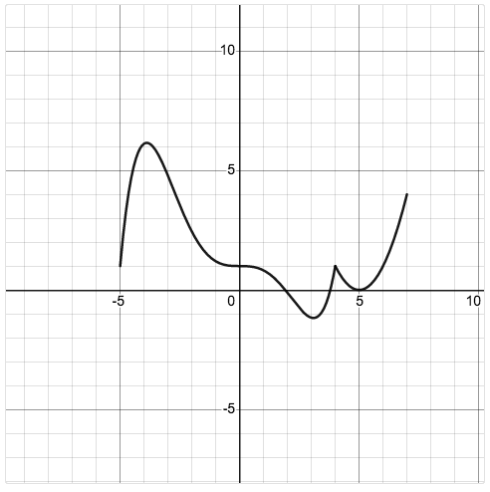
\includegraphics [scale= .4]{4_1_g1}
\end{minipage}


\item Sketch a graph of a function that has exactly one critical point at $x=2$ and exactly one inflection point at $x=4$, or explain why no such function exists.\\
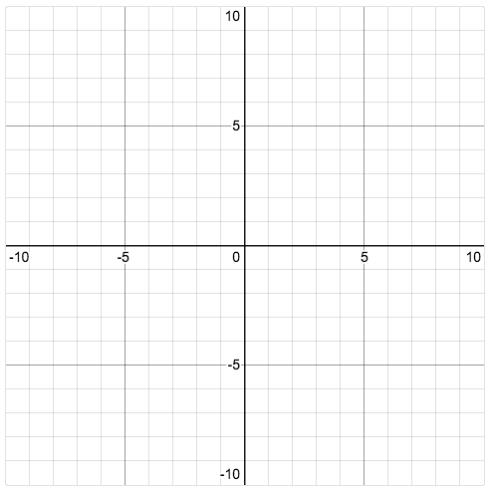
\includegraphics [scale =.4]{4_1_g2}

\newpage

$\hspace{10px}$ \\

\item The graph of the DERIVATIVE, $f'$ is shown. 

\noindent\begin{minipage}{0.45\textwidth}% adapt widths of minipages to your needs
(a) What are the critical points of $f$? (NOT $f'$).\\
\vspace{10mm}\\
(b) Where does $f$ have a local max? A local min?\\
\vspace{10mm}\\
(c) What are the inflection points of $f$? (NOT $f'$).\\
\vspace{10mm}\\

\end{minipage}%
\hspace{5mm}
\begin{minipage}{0.3\textwidth}
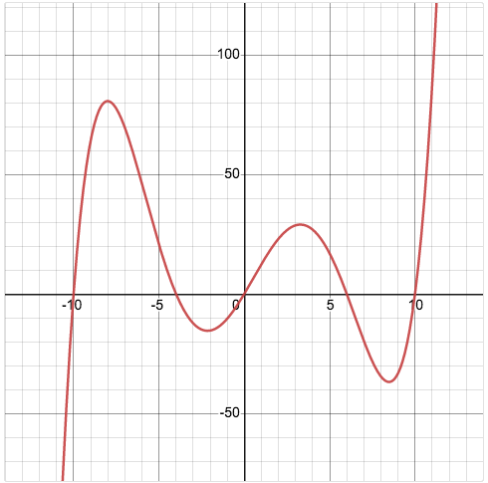
\includegraphics [scale= .4]{4_1_g3}
\end{minipage}



\item Let  $\displaystyle f(x)=\frac{a}{x^{2}}+x$.
	\begin{enumerate}
	\item If a is $a$ nonzero constant, find all critical points of $f$.
	\vfill
	\item Use the second‐derivative test to show that if $a$ is positive then the graph has a local minimum, and if $a$ is negative then the graph has a local maximum.
	\vfill
	\vfill
	\item Check your work by graphing $f$ in Desmos.
	\end{enumerate}

\item The rabbit population on a small Pacific island is approximated by

$$P=\frac{2000}{1+e^{\left(5.3-0.4t\right)}}$$

with $t$ measured in years since 1774, when Captain James Cook left 10 rabbits on the island.
	\begin{enumerate}
	\item Graph $P$ on Desmos. Does the population level off?
	\vfill
	\item Estimate when the rabbit population grew most rapidly. How large was the population at that time?
	\vfill
	\item What natural causes could lead to the shape of the graph of $P$?
	\vfill
	\end{enumerate}

\end{enumerate}
\end{document} 

%%%%%%%%%
\begin{tcolorbox}
\textbf{Warm-up: } Solve the following equations for $t$.
\begin{multicols}{2}
\begin{enumerate}
\item $(t+1)^2=9$
\item $tx+x^2=5$
\end{enumerate}
\end{multicols}
\end{tcolorbox}

MINIPAGE
\noindent\begin{minipage}{0.3\textwidth}% adapt widths of minipages to your needs
try 1
\end{minipage}%
\hspace{40mm}
\begin{minipage}{0.6\textwidth}
a) $f'(2)=$\\\

b) $f'(4)=$\\

c) $f'(6)=$\\

d) $f'(7)=$\\

e) $f'(8)=$
\end{minipage}
